\chapter{Heredity and Traits}\label{ch:g9:heredity-and-traits}

Family photographs are \omterm{def:g1:living-or-not:living}{biology} data. Grandmother's chin on
the toddler, the mother's curls on neither child, one
brother tall and one not --- resemblance runs in families,
and so does difference. This book has leaned on the fact for
years (\cref{rem:g4:animal-reproduction:mix}'s foal,
\cref{prop:g8:sexual-reproduction:shuffle}'s siblings);
this year's opening chapter finally studies it: what exactly
is inherited, what is not, and what the patterns of family
resemblance let us conclude.

\begin{omfigure}
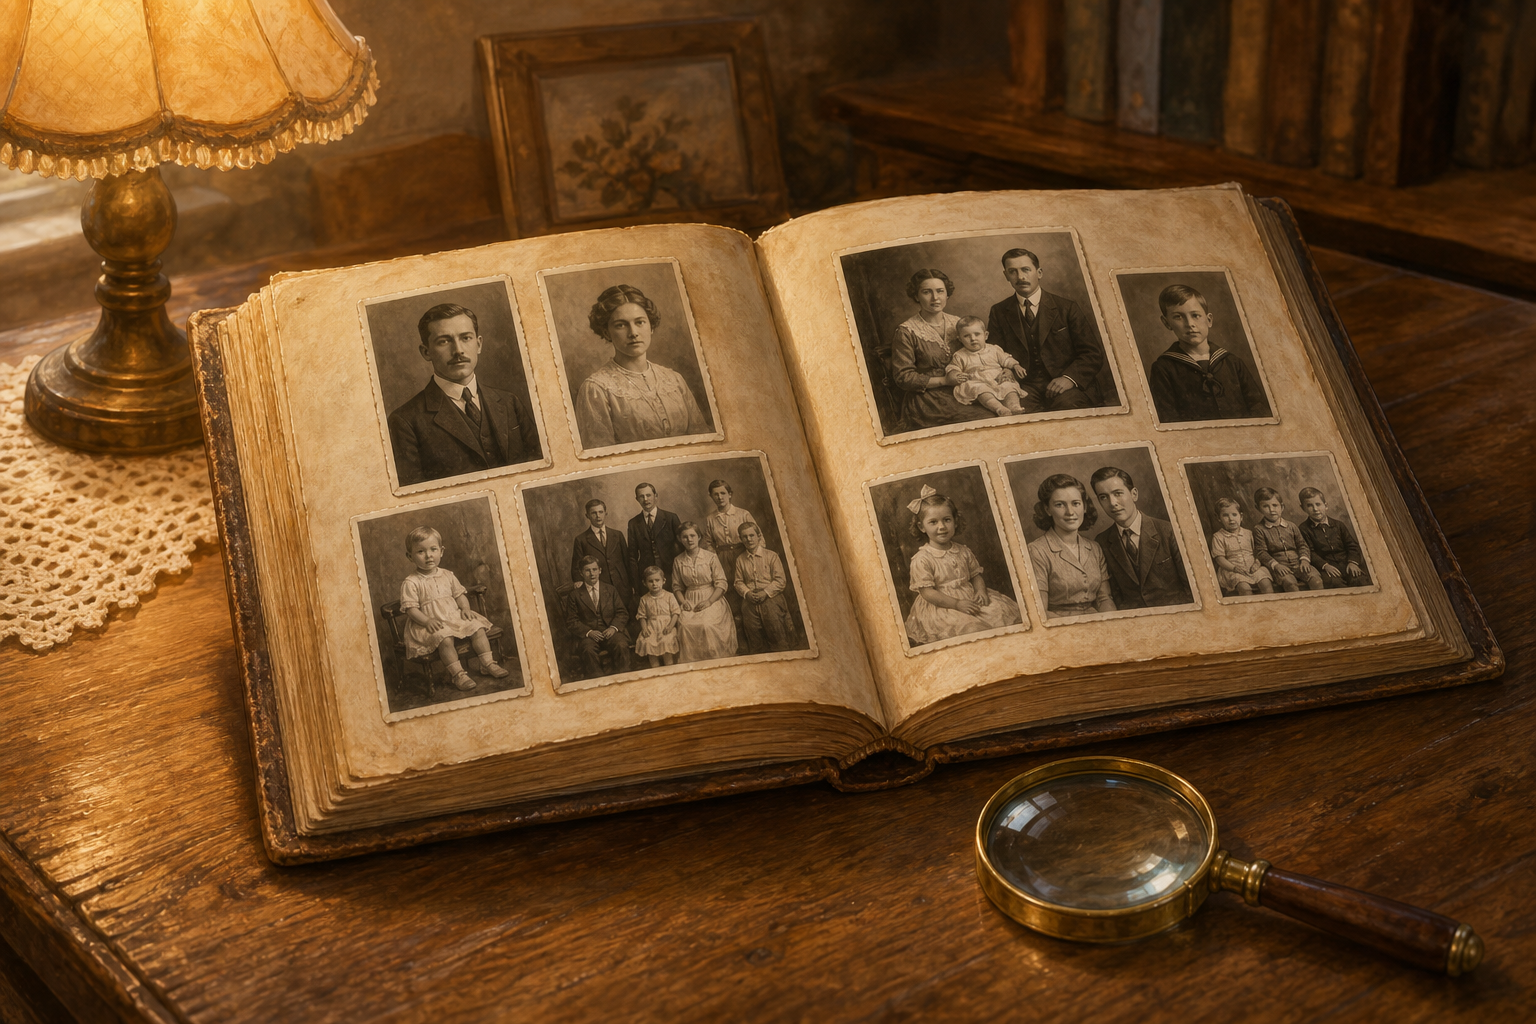
\includegraphics[width=0.62\linewidth]{images/book1/ai/g9-family-album.png}

{\small \omterm{def:g1:living-or-not:living}{Biology} data, sepia edition: resemblance and
difference, running down the generations.}
\end{omfigure}

\section{Traits, and where they come from}

\begin{definition}[Traits]\label{def:g9:heredity-and-traits:traits}
A \emph{trait}\index{trait} is any describable
characteristic of an individual: \omterm{def:g1:the-five-senses:sense}{eye} color, \omterm{prop:g4:journey-of-food:absorb}{blood} group,
earlobe shape, height, a singing voice, a scar. The
individual's whole collection of traits is built by two
workings: what was \emph{inherited}, and what the
\emph{\omterm{def:g6:exploring-our-environment:components}{environment} and life} added
(\cref{def:g4:adapted-to-their-world:adaptation}'s world,
acting on one body).
\end{definition}

\begin{definition}[Heredity]\label{def:g9:heredity-and-traits:heredity}
\emph{Heredity}\index{heredity} is the transmission of
\omterm{def:g9:heredity-and-traits:traits}{traits} from parents to offspring through reproduction ---
through, as \cref{ch:g8:sexual-reproduction} showed, two
single \omterm{def:g5:first-look-at-cells:cell}{cells}. \omterm{def:g9:heredity-and-traits:traits}{Traits} that pass this way are
\emph{hereditary}\index{hereditary trait}: \omterm{def:g1:the-five-senses:sense}{eye} color and
\omterm{prop:g4:journey-of-food:absorb}{blood} group are; scars and pierced \omterm{def:g1:the-five-senses:sense}{ears} are not, however
long worn. The sorting test is the \omterm{def:g8:sexual-reproduction:gametes}{gametes}: what two \omterm{def:g5:first-look-at-cells:cell}{cells}
cannot carry, families cannot transmit.
\end{definition}

\begin{example}[Sorting a family album]\label{ex:g9:heredity-and-traits:album}
Grandfather's photographs: his distinctive nose ---
\omterm{def:g9:heredity-and-traits:heredity}{hereditary}, there it is again on the aunt and the cousin;
his weathered farmer's tan --- acquired, his
office-working grandson lacks it; his height --- partly
both, for the grandson overtops him on the same frame,
fed by richer years (\cref{prop:g3:balanced-diet:jobs});
his violin skill --- not \omterm{def:g9:heredity-and-traits:heredity}{hereditary} as skill
(\cref{ex:g8:nervous-communication:juggler}: \omterm{def:g8:nervous-communication:synapse}{synapses} are
trained, not transmitted), though the musical family
tells us something subtler is at work in what is passed
on: perhaps aptitude, never the trained wiring itself.
\end{example}

\begin{proposition}[Inherited and acquired]\label{prop:g9:heredity-and-traits:sorting}
The two workings separate on three tests:
\begin{enumerate}
  \item \emph{family pattern}: \omterm{def:g9:heredity-and-traits:heredity}{hereditary traits} recur
        through the tree along reproduction's lines;
        acquired ones follow lives (all the sailors
        weathered, whoever their parents);
  \item \emph{presence from the start}: \omterm{prop:g4:journey-of-food:absorb}{blood} group is
        fixed at \omterm{def:g5:flower-to-fruit:steps}{fertilization}; the tan and the skill are
        built after;
  \item \emph{transmission}: children of amputees have
        their \omterm{def:g1:my-body:parts}{limbs}; children of bodybuilders start
        untrained. Acquired \omterm{def:g9:heredity-and-traits:traits}{traits} die with their
        acquirer --- the \omterm{def:g8:sexual-reproduction:gametes}{gametes} do not carry them.
\end{enumerate}
Most visible \omterm{def:g9:heredity-and-traits:traits}{traits} --- height, build, even temperament
--- are woven of both workings, inherited range and lived
filling-in.
\end{proposition}
\admitted

\section{Reading family patterns}

\begin{example}[Traits that skip]\label{ex:g9:heredity-and-traits:skip}
Some patterns puzzle at first sight: two brown-eyed
parents with a blue-eyed child; grandmother's \omterm{def:g9:heredity-and-traits:traits}{trait}
absent in every child yet returning in a grandchild.
Skipping is common, and it carries a heavy conclusion: a
parent can \emph{transmit what they do not show}. The
\omterm{def:g9:heredity-and-traits:traits}{trait}'s instructions traveled hidden through a generation
--- so what is inherited is not the \omterm{def:g9:heredity-and-traits:traits}{trait} itself but
something that \emph{determines} it, carriable unseen.
\end{example}

\begin{proposition}[What the patterns force us to conclude]\label{prop:g9:heredity-and-traits:conclusions}
Three conclusions, each forced by an observation:
\begin{enumerate}
  \item since acquired \omterm{def:g9:heredity-and-traits:traits}{traits} do not pass, what passes
        must be \emph{determinants} --- instructions for
        building \omterm{def:g9:heredity-and-traits:traits}{traits}, not the \omterm{def:g9:heredity-and-traits:traits}{traits} themselves;
  \item since \omterm{def:g9:heredity-and-traits:traits}{traits} skip generations, the determinants
        can be \emph{carried without showing}: each
        individual carries more than it displays;
  \item since every child receives from both parents by
        two \omterm{def:g8:sexual-reproduction:gametes}{gametes}
        (\cref{prop:g8:sexual-reproduction:core}), each
        parent contributes a \emph{selection} of its
        determinants --- and the selections differ from
        child to child, or siblings would match
        (\cref{prop:g8:sexual-reproduction:shuffle}'s
        shuffle, now located: it is a shuffle \emph{of
        determinants}).
\end{enumerate}
\end{proposition}
\admitted

\begin{remark}[The question this sets]\label{rem:g9:heredity-and-traits:question}
The family album has cornered us into a marvelous
question. Somewhere in a \omterm{def:g8:reproductive-systems:male}{sperm cell}'s almost-nothing
(\cref{ex:g8:reproductive-systems:sperm} --- a packed
\omterm{def:g6:cell-unit-of-life:parts}{nucleus} and a tail) travel instructions for a nose, a
\omterm{prop:g4:journey-of-food:absorb}{blood} group, an \omterm{def:g1:the-five-senses:sense}{eye} color --- carriable unshown,
selectable by halves, readable by the growing body.
\emph{Where are they, and what are they made of?} The
sperm's anatomy already points the answer: everything the
father sends fits in a \omterm{def:g6:cell-unit-of-life:parts}{nucleus}
(\cref{rem:g5:first-look-at-cells:nucleus} promised that
spot mattered). The next two chapters open it.
\end{remark}

\begin{method}[Auditing a trait]\label{met:g9:heredity-and-traits:audit}
For any \omterm{def:g9:heredity-and-traits:traits}{trait}, run the three tests:
\begin{enumerate}
  \item map it on the family tree: does it follow
        reproduction's lines, or lives and habits?
  \item date it: fixed from the start, or built along the
        way?
  \item apply the \omterm{def:g8:sexual-reproduction:gametes}{gamete} test: could two \omterm{def:g5:first-look-at-cells:cell}{cells} carry it?
        (a scar cannot; a \omterm{prop:g4:journey-of-food:absorb}{blood} group can);
  \item verdict: inherited, acquired, or --- commonest
        --- an inherited range, lived into.
\end{enumerate}
\end{method}

\section{Exercises}

\begin{exercise}[$\star$]\label{exo:g9:heredity-and-traits:1}
Define \omterm{def:g9:heredity-and-traits:traits}{trait} and \omterm{def:g9:heredity-and-traits:heredity}{heredity}, and give the sorting test in
one phrase.
\end{exercise}

\begin{exercise}[$\star$]\label{exo:g9:heredity-and-traits:2}
Classify: \omterm{prop:g4:journey-of-food:absorb}{blood} group; a pierced \omterm{def:g1:the-five-senses:sense}{ear}; freckles; fluent
French; earlobe shape.
\end{exercise}

\begin{exercise}[$\star$]\label{exo:g9:heredity-and-traits:3}
State the three tests of
\cref{prop:g9:heredity-and-traits:sorting}.
\end{exercise}

\begin{exercise}[$\star$]\label{exo:g9:heredity-and-traits:4}
Why do children of bodybuilders start untrained? What
does that show?
\end{exercise}

\begin{exercise}[$\star$]\label{exo:g9:heredity-and-traits:5}
What does a skipping \omterm{def:g9:heredity-and-traits:traits}{trait} prove a parent can do?
\end{exercise}

\begin{exercise}[$\star$]\label{exo:g9:heredity-and-traits:6}
Why must what is inherited be determinants rather than
\omterm{def:g9:heredity-and-traits:traits}{traits}? One sentence.
\end{exercise}

\begin{exercise}[$\star\star$]\label{exo:g9:heredity-and-traits:7}
Height ran taller in the grandson on the same frame.
Untangle the two workings in that sentence.
\end{exercise}

\begin{exercise}[$\star\star$]\label{exo:g9:heredity-and-traits:8}
Explain why siblings differ, in determinant language ---
and why identical twins
(\cref{exo:g8:from-egg-to-birth:10}) do not.
\end{exercise}

\begin{exercise}[$\star\star$]\label{exo:g9:heredity-and-traits:9}
Run \cref{met:g9:heredity-and-traits:audit} on: (a) a
family's recurring early gray hair; (b) a football
player's stamina.
\end{exercise}

\begin{exercise}[$\star\star$]\label{exo:g9:heredity-and-traits:10}
The violin case: what could the musical family be
transmitting, if never the trained skill? Distinguish
carefully.
\end{exercise}

\begin{exercise}[$\star\star$]\label{exo:g9:heredity-and-traits:11}
Two brown-eyed parents, a blue-eyed child --- and the
neighbor doubts the family. Defend the family with
\cref{ex:g9:heredity-and-traits:skip}'s logic.
\end{exercise}

\begin{exercise}[$\star\star\star$]\label{exo:g9:heredity-and-traits:12}
From the \omterm{def:g8:reproductive-systems:male}{sperm cell}'s anatomy alone
(\cref{ex:g8:reproductive-systems:sperm}), argue where
the father's determinants must sit --- and what size
that implies for the instructions of a whole human.
\end{exercise}

\section{Problem: The Village Genealogist}

\begin{problem}[{Weekend problem --- three generations,
one trait ledger}]\label{pb:g9:heredity-and-traits:1}
A village genealogist annotates the parish's family
trees with \omterm{def:g9:heredity-and-traits:traits}{traits}: the ``chapel chin'' (a distinctive
chin recurring for a century), left-handedness, the
bakers' floury \omterm{def:g7:how-animals-breathe:four}{lung} cough, \omterm{prop:g4:journey-of-food:absorb}{blood} groups from the
donation register, and the shepherds' weathered faces.

\medskip\noindent\textbf{Part I --- Sorting the
ledger.}
\begin{enumerate}
  \item Sort the five \omterm{def:g9:heredity-and-traits:traits}{traits} by
        \cref{met:g9:heredity-and-traits:audit}, with
        the deciding test for each.
  \item The cough follows the bakery, not the family:
        marrying in brings it, moving away loses it.
        Which test is this, in action?
  \item The chapel chin skips the middle generation in
        two \omterm{def:g1:plants-around-us:tree}{branches}. Draw the conclusion it forces.
  \item \omterm{prop:g4:journey-of-food:absorb}{Blood} groups sometimes surprise the register: a
        group-O child of group-A and group-B parents.
        What must each parent have carried?
\end{enumerate}

\medskip\noindent\textbf{Part II --- The determinant
reading.}
\begin{enumerate}[resume]
  \item Rewrite the chin's century in determinant
        language: what actually traveled down four
        generations, in what vehicles
        (\cref{def:g9:heredity-and-traits:heredity})?
  \item Why do the chin-carrying cousins differ in
        everything else? Locate the shuffle.
  \item The genealogist finds no case --- in a century
        --- of a scar, a trade or a language passing to
        a newborn. State the generalization, and its
        mechanism-level reason.
  \item One family's twins match to the chin and beyond.
        What does the ledger conclude about their
        beginning
        (\cref{rem:g5:human-reproduction:twins})?
\end{enumerate}

\medskip\noindent\textbf{Part III --- The lecture.}
\begin{enumerate}[resume]
  \item The genealogist lectures: ``the parish transmits
        two inheritances --- one by \omterm{def:g8:sexual-reproduction:gametes}{gametes}, one by
        living together.'' Assign the ledger's five
        \omterm{def:g9:heredity-and-traits:traits}{traits} to the two channels.
  \item ``Each of us displays less than we carry.''
        Defend from the ledger, twice.
  \item A listener asks what the \omterm{def:g8:sexual-reproduction:gametes}{gamete} channel's
        instructions are physically. Give the honest
        answer of \cref{rem:g9:heredity-and-traits:question}
        --- location known, contents next chapter.
  \item Close the lecture with the audit's one-line
        verdict on the commonest case: most \omterm{def:g9:heredity-and-traits:traits}{traits} are
        \emph{what}, lived \emph{how}?
\end{enumerate}
\end{problem}
